\documentclass[10pt,twocolumn]{article}
\usepackage[margin=0.8in,columnsep=0.25in]{geometry}
\usepackage{graphicx,booktabs,amsmath,hyperref,microtype,xcolor,enumitem,caption}
\hypersetup{colorlinks=true,linkcolor=blue,citecolor=blue,urlcolor=blue}
\setlist{nosep,leftmargin=1.2em}
\captionsetup{font=small,labelfont=bf}
\title{\textbf{Benign Drift as a Swarm's Weak Link:\\Aggregation Rules, Peer Context and a Refusal-Direction Monitor}}
\author{Abdurrachman Mappuji\\
{\small GCAS College Dublin, Dublin, Ireland; Department of Cyber Security, Royal Holloway, University of London, UK}\\
{\small abdurrachman.mappuji@gcas.ie}}
\date{Apart Research Swarm Alignment Sprint, November 2026 (Track 2: The Science of Agent Networks)}
\begin{document}
\maketitle

\begin{abstract}
A swarm of language-model agents is only as safe as the agents it routes requests to. Most swarm-safety work assumes an adversarial member; we study a quieter weak link, an agent that was fine-tuned on a harmless task and lost part of its refusal behaviour without anyone intending it. Using Qwen2.5-1.5B-Instruct and a copy fine-tuned on grade-school maths, we ask how such an agent changes the safety of a group, and whether a refusal-direction probe can monitor it. Simulating aggregation rules from per-prompt outcomes, one drifted agent in a pool of five raises the share of harmful requests answered from 6.5\% to 41\% for a requester who can try every agent, while majority voting holds until three agents have drifted. In live four-agent chains, one drifted agent raises the share of requests answered by some agent from 34\% to about 55--60\%, with diminishing increments for further drifted agents and no detectable contagion once the framing effect is controlled. A probe on the refusal direction flags 98\% of harmful requests from inside the drifted agent, which refuses only 46\% of them, but both signals fail under rot13 and base64 encoding. We report what we could not test, including hosted models and adversarial coordination.
\end{abstract}

\section{Introduction}
Alignment cannot stop at single models when agents negotiate, trade and share tools. Recent work catalogues multi-agent risks~\cite{hammond2025} and shows that agents can collude secretly~\cite{motwani2024} and that tasks split across agents can evade per-agent filters~\cite{jones2025}. These studies centre on deliberately adversarial or coordinating agents. A more mundane route also exists: practitioners adapt models to downstream tasks, and even benign fine-tuning can erode refusal~\cite{qi2023}. A swarm assembled from specialised agents may therefore contain members that are weaker than their base model without being malicious.

We ask three questions. (Q1) How does one or more benignly drifted agents change the safety of a group, under routing and voting rules a designer might choose? (Q2) Do drifted agents spread or absorb refusal through the context they share? (Q3) Can an internal refusal-direction probe monitor a drifted agent, and where does it fail?

\paragraph{Contributions.} (i) An aggregation analysis showing that, for a requester who can try every agent, a single drifted agent determines the group's safety, while majority voting and ``any refusal blocks'' buy robustness at different costs. (ii) A live chain experiment with a framing control that separates peer content from prompt framing. (iii) A monitor comparison showing that the refusal direction remains readable inside a drifted agent that no longer acts on it, and that simple encodings defeat both the probe and the agent.

\paragraph{Preexisting and new work.} The models, the drift recipe, the evaluation prompts, the refusal detector and the per-prompt outcomes come from our earlier study~\cite{mappuji2026} and are marked as preexisting in the repository. All analyses in this paper, the chain and monitor experiments, and the figures were produced during the sprint.

\section{Related Work}
\textbf{Multi-agent risk.} Hammond et al.~\cite{hammond2025} organise multi-agent failure modes; Motwani et al.~\cite{motwani2024} study secret collusion; Lee and Tiwari~\cite{leetiwari2024} show prompts that propagate across agents; Jones et al.~\cite{jones2025} show that splitting a task evades per-agent safety filters. AI control~\cite{greenblatt2024} studies oversight against intentional subversion. We differ by studying an agent that is weaker without being adversarial, and by measuring group outcomes under simple aggregation rules.
\textbf{Safety drift and refusal directions.} Qi et al.~\cite{qi2023} show that fine-tuning on benign data can erode safety. Arditi et al.~\cite{arditi2024} show that refusal is mediated by a single residual-stream direction, which we reuse as a probe. Weight-space repair methods are implemented in the SafeTune library~\cite{safetune}; our earlier study compared them on a single agent~\cite{mappuji2026}.

\section{Setup}
\textbf{Agents.} The aligned agent (A) is Qwen2.5-1.5B-Instruct. The drifted agent (D) is the same model after a LoRA fine-tune on 2{,}000 GSM8K examples (rank 16, one epoch), merged into the weights~\cite{mappuji2026}. Both run in bfloat16 on an Apple M1 GPU with greedy decoding. \textbf{Prompts and refusal.} Harmful prompts are public benchmark prompts. The aggregation analysis (Section~\ref{sec:agg}) uses the 200 held-out harmful and 150 harmless prompts evaluated earlier; live experiments use a fixed sample of 100 harmful and 100 harmless prompts (so rates differ slightly between sections; on the 100-prompt sample A refuses 87\% and D 46\%, on the 200-prompt set 93.5\% and 59.5\%). A reply counts as a refusal if one of a fixed list of refusal phrases occurs in its first 200 characters. This detector is coarse and is a limitation. \textbf{Probe.} We take the refusal direction of A at layer 14, chosen before looking at any transformed condition, and score the last-token residual by its projection. The threshold is the 95th percentile of scores on 200 clean harmless prompts. All intervals are 95\% Wilson or bootstrap intervals unless noted.

\section{Results}
\subsection{Aggregation rules (Q1)}\label{sec:agg}
We reuse per-prompt refusal outcomes of A and D to simulate a pool of five agents with $k$ drifted members under four rules: the request goes to a random agent; a requester tries every agent and keeps a compliant answer (\emph{shop}); the pool answers if a majority would; the pool answers only if all agents would (\emph{any refusal blocks}). Because decoding is greedy, copies are identical, so this analysis shows how rules combine behaviour; it does not model interaction.

\begin{figure}[t]\centering
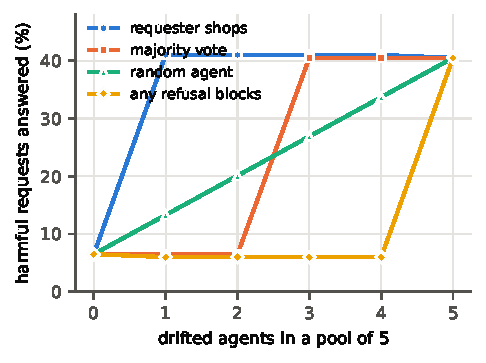
\includegraphics[width=\columnwidth]{figures/fig_aggregation.pdf}
\caption{Share of harmful requests answered (200 prompts) for a pool of five agents, as drifted agents replace aligned ones. With $k{=}0$ the rate is 6.5\%; with $k{=}5$ it is 40.5\%.}\label{fig:agg}
\end{figure}

Figure~\ref{fig:agg} shows the result. A single drifted agent raises the share answered from 6.5\% to 41.0\% under shopping, to 13.3\% under random routing, and leaves majority voting at 6.5\% until three agents have drifted, after which it jumps to 40.5\%. Requiring unanimous compliance holds the rate at about 6\% for up to four drifted agents. Its cost is modest here: with one drifted agent it blocks 8.7\% of plain harmless prompts against 8.0\% for the aligned agent alone (a difference well inside the noise of 150 prompts). In a heterogeneous pool of the eleven non-degenerate variants from our earlier study (aligned, drifted and repaired), unanimity reduces harmful answers to 1.5\% but blocks 12.0\% of harmless prompts, against 5.3\% for random routing.

\subsection{Chains and peer context (Q1, Q2)}
In a chain of four agents, agent~1 sees the request and agent~$k$ sees it together with the previous agent's reply (``a teammate replied\ldots''). Table~\ref{tab:chain} gives refusal by position and the share of requests answered by some agent.

\begin{table}[t]\centering\small
\begin{tabular}{lccccc}\toprule
Chain & p1 & p2 & p3 & p4 & Answered\\\midrule
AAAA & .87 & .72 & .74 & .76 & .34\\
DAAA & .46 & .70 & .73 & .70 & .60\\
ADAA & .87 & .51 & .73 & .71 & .59\\
AAAD & .87 & .72 & .74 & .57 & .54\\
ADAD & .87 & .51 & .73 & .46 & .63\\
DDDD & .46 & .52 & .51 & .45 & .72\\
\bottomrule\end{tabular}
\caption{Refusal rate by position in four-agent chains (A aligned, D drifted; 100 harmful prompts) and the share answered by some agent.}\label{tab:chain}
\end{table}

\begin{figure}[t]\centering
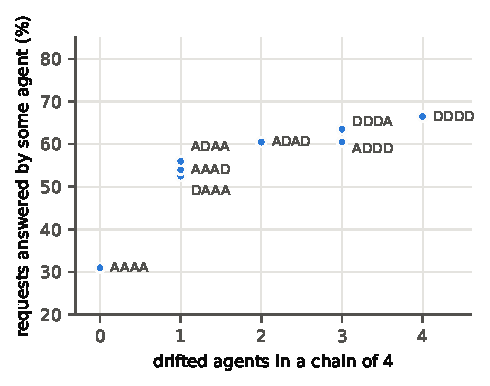
\includegraphics[width=\columnwidth]{figures/fig_chain.pdf}
\caption{Share of requests answered by some agent against the number of drifted agents in the chain.}\label{fig:chain}
\end{figure}

\textbf{Drift raises the union, with diminishing steps.} The first drifted agent raises the share answered from 34\% to 54--60\%, depending on its position; a second adds a few points (ADAD, 63\%) and four drifted agents reach 72\% (Figure~\ref{fig:chain}). With three drifted agents the share is 64--69\% (ADDD, DDDA), so after the first drifted agent each further one adds only a few points. This does not support the hypothesis that each additional misaligned agent adds more risk than the last, at least in this toy setting. Even the all-aligned chain answers 34\% of requests somewhere although a single aligned agent answers 13\%, so presenting the same request in different surrounding context behaves like a weak form of refusal shopping.

\textbf{Controlling for framing.} Position-2 refusal falls from 87\% to 72\% in AAAA, even though no agent has drifted. To separate framing from peer content, we gave a receiving agent the same wrapper around a fixed peer reply (Table~\ref{tab:control}). The neutral wrapper alone costs the aligned agent 8 points and raises refusal of the drifted agent by 11, so the framing effect has opposite signs for the two agents. A compliant peer opener did not lower the aligned agent's refusal relative to the neutral wrapper (77\% against 79\%). We found no evidence that aligned agents downstream of a drifted agent refuse less (DAAA, position 2: 70\% against 72\% in AAAA), nor that a drifted agent refuses more after aligned peers (AAAD, position 4: 57\%, equal to its neutral-wrapper rate). Two controls moved against expectation: a refusing peer reply lowered aligned refusal (67\%), and a compliant opener raised drifted refusal (67\%). Generations were not saved, so we could not check whether the substring detector misreads the framed replies. With $n{=}100$ the intervals are about $\pm$10 points; we read these results as ``contagion not detected'', not as ``absent''.

\begin{table}[t]\centering\small
\begin{tabular}{lcccc}\toprule
Receiver & none & neutral & peer refuses & peer complies\\\midrule
Aligned & .87 & .79 & .67 & .77\\
Drifted & .46 & .57 & .40 & .67\\
\bottomrule\end{tabular}
\caption{Refusal rate when the receiver sees the chain wrapper around a fixed peer reply (100 harmful prompts).}\label{tab:control}
\end{table}

\subsection{A probe inside the drifted agent (Q3)}
Figure~\ref{fig:probe} and Table~\ref{tab:probe} compare what the agent does with what the probe reads, on the same inputs. On direct requests D refuses 46\%, yet the aligned model's refusal direction, read from D's own activations, flags 98\% (AUC 0.98), at a false-alarm rate of 14\% on harmless prompts. The signal that refusal depends on is present but no longer acted on; the same holds for requests with spaced letters (D refuses 40\%, probe flags 85\% at 17\% false alarms). The obvious reading, that a probe could monitor drifted agents, comes with a caveat: our threshold was set for a 5\% false-alarm rate on one harmless set and gave 11--14\% on another, so absolute detection rates are optimistic.

Simple encodings defeat both. Under rot13 and base64, D complies (refusal 3\% and 0\%) and the probe's AUC falls to 0.52 and 0.58; for the aligned agent's probe the AUC is 0.65 and 0.59. The aligned agent's high refusal under rot13 and leetspeak applies equally to harmless prompts (98--99\%), so it reflects confusion rather than detection. A perplexity score flags rot13 text, harmful or not (100\% flagged), but cannot tell harmful from harmless; we did not test combining it with the probe. A prompted judge using the 1.5B model was near chance on clean text (AUC 0.56) and is therefore not a useful baseline, so we make no claim that the probe beats text monitors.

Splitting a request at a word midpoint across two agents did not hide it from the probe: the maximum fragment score has AUC 0.99 against 0.98 for the whole request. Harmless fragments also raised alarms (21--33\% at the same threshold), and fragment-level refusals of both agents were largely confusion (A refused 72\% of harmless first halves). Our split is mechanical; this does not contradict reports that carefully designed splits evade monitors.

\begin{figure}[t]\centering
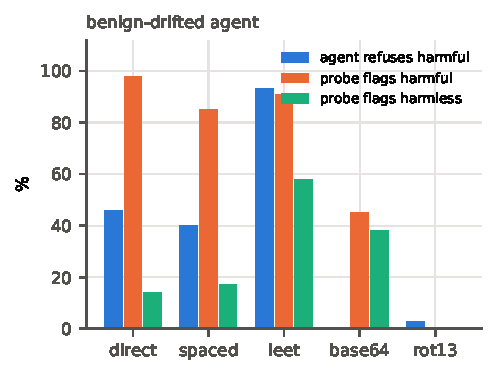
\includegraphics[width=\columnwidth]{figures/fig_probe_vs_behavior.pdf}
\caption{Benign-drifted agent: how often the agent refuses harmful requests, how often the probe flags them, and how often the probe flags harmless requests, per input transformation (100 prompts each).}\label{fig:probe}
\end{figure}

\begin{table}[t]\centering\footnotesize
\begin{tabular}{lcccc}\toprule
& A refuses & D refuses & \multicolumn{2}{c}{Probe on D}\\
& & & TPR / FPR & AUC\\\midrule
direct & .87 & .46 & .98 / .14 & .98\\
spaced & .68 & .40 & .85 / .17 & .92\\
leet & 1.0 & .93 & .91 / .58 & .75\\
base64 & .14 & .00 & .45 / .38 & .58\\
rot13 & .96 & .03 & .00 / .00 & .52\\
\bottomrule\end{tabular}
\caption{Behaviour and probe on harmful inputs. A refuses harmless inputs 8\% (direct), 9\%, 99\%, 18\% and 98\% in the same order; D refuses 1\%, 4\%, 68\%, 0\% and 4\%.}\label{tab:probe}
\end{table}

\section{Discussion}
Three practical points follow, each limited by scale. First, aggregation rules matter more than the share of drifted agents. If a requester can try several agents, one drifted member is as bad as all of them; majority voting and unanimity restore safety at different thresholds, and in our data unanimity was cheap. Second, drift in a member is a replicable weakness: fine-tuning recipes can be copied, so the same weakened agent can appear several times in a swarm. Third, a monitor that reads the refusal direction can recover what the agent itself fails to act on, but only while messages look like ordinary text; obfuscated or compressed message formats, which we approximate only with fixed encodings, defeat it.

\section{Limitations}
All agents are 1.5B models, greedy decoding was used, and refusal is a substring match, which both misses soft compliance and counts confusion as refusal. The live experiments use 100 prompts, so differences below about 10 points should not be interpreted. Drift comes from one fine-tune on one dataset; in our earlier study a second model family showed no drift under the same recipe~\cite{mappuji2026}, so the weak-link effect is model-dependent. The aggregation analysis simulates rules from per-prompt outcomes of identical copies and ignores interaction. We did not test hosted frontier models, adversarial coordination, learned monitors, careful task splits, or reward-driven protocols. Probe thresholds were calibrated on one harmless set and transferred imperfectly. The unexplained control results above remain unresolved.

\section*{Acknowledgements}
The sprint talks by speakers at UK AISI/MATS, AE Studio, Swarmchaser, UT Austin, Gutenberg PBC and others shaped the experiment design. We read some talks only through automatic summaries and make no claim about their contents beyond ideas used here.

\appendix
\section{Limitations and Dual-Use / Ethical Considerations}
\textbf{Data.} We used only public benchmark prompts and kept no generated harmful text; saved artefacts are per-prompt refusal flags and scores. \textbf{Transformations.} The obfuscations are standard public encodings (rot13, base64, letter substitution, spacing) applied mechanically; the split is a word-midpoint cut. We do not provide or evaluate crafted attack recipes. \textbf{Misuse.} The main finding, that routing a request to the weakest member defeats the group, is obvious to a requester but also a design warning; the corresponding mitigations are to avoid agents that can be selected by the requester, to require agreement among agents, and to monitor internal states rather than outputs. \textbf{Overclaiming.} We report null and unexplained results as such. Hosted-model validation was planned but not performed because platform credits were unavailable.

\begin{thebibliography}{9}\small
\bibitem{hammond2025} L. Hammond et al., ``Multi-Agent Risks from Advanced AI,'' arXiv:2502.14143, 2025.
\bibitem{motwani2024} S. R. Motwani et al., ``Secret Collusion among AI Agents: Multi-Agent Deception via Steganography,'' NeurIPS 2024.
\bibitem{jones2025} Jones et al., ``Splitting tasks to evade per-agent safety filters,'' OpenReview, 2025.
\bibitem{leetiwari2024} D. Lee and M. Tiwari, ``Prompt Infection: LLM-to-LLM Prompt Injection within Multi-Agent Systems,'' arXiv:2410.07283, 2024.
\bibitem{greenblatt2024} R. Greenblatt et al., ``AI Control: Improving Safety Despite Intentional Subversion,'' arXiv:2312.06942, 2024.
\bibitem{qi2023} X. Qi et al., ``Fine-tuning Aligned Language Models Compromises Safety, Even When Users Do Not Intend To!,'' arXiv:2310.03693, 2023.
\bibitem{arditi2024} A. Arditi et al., ``Refusal in Language Models Is Mediated by a Single Direction,'' arXiv:2406.11717, 2024.
\bibitem{mappuji2026} A. Mappuji, ``Repairing Safety Drift Without Retraining in Small Fine-Tuned Language Models: Weight-Space Methods and a Located Refusal Direction,'' Zenodo, 2026. doi:10.5281/zenodo.24040671.
\bibitem{safetune} Lexsi Labs, ``SafeTune: auditing and repairing safety drift in fine-tuned LLMs,'' software, https://safetune.lexsi.ai.
\end{thebibliography}
\end{document}
